\documentclass{sigchi-ext}
% Please be sure that you have the dependencies (i.e., additional
% LaTeX packages) to compile this example.
\usepackage[T1]{fontenc}
\usepackage{textcomp}
\usepackage[scaled=.92]{helvet} % for proper fonts
\usepackage{graphicx} % for EPS use the graphics package instead
\usepackage{balance}  % for useful for balancing the last columns
\usepackage{booktabs} % for pretty table rules
\usepackage{ccicons}  % for Creative Commons citation icons
\usepackage{ragged2e} % for tighter hyphenation

% Some optional stuff you might like/need.
% \usepackage{marginnote}
% \usepackage[shortlabels]{enumitem}
% \usepackage{paralist}
% \usepackage[utf8]{inputenc} % for a UTF8 editor only

%% OVERRIDE THE DEFAULT COPYRIGHT STRIP
\copyrightinfo{Permission to make digital or hard copies of part or all of this work for personal or classroom use is granted without fee provided that copies are not made or distributed for profit or commercial advantage and that copies bear this notice and the full citation on the first page. Copyrights for third-party components of this work must be honored. For all other uses, contact the Owner/Author.\\
Copyright is held by the owner/author(s).\\
{\emph{TEI'17}}, March 20-23, 2017, Yokohama, Japan.\\
ACM XXX-X-XXXX-XXXX-X/XX/XX\\
\url{http://dx.doi.org/XX.XXXX/XXXXXXX.XXXXXXX}}

% Paper metadata (use plain text, for PDF inclusion and later
% re-using, if desired).  Use \emtpyauthor when submitting for review
% so you remain anonymous.
\def\plaintitle{Musical Skin: A Fabric Interface for Expressive Interaction}
  \def\plainauthor{First Author, Second Author, Third Author}
\def\emptyauthor{}
\def\plainkeywords{Authors' choice; of terms; separated; by
  semicolons; include commas, within terms only; required.}
\def\plaingeneralterms{Documentation, Standardization}

\title{Musical Skin: A Cloth Interface for Expressive Music Control}

\numberofauthors{3}
% Notice how author names are alternately typesetted to appear ordered
% in 2-column format; i.e., the first 4 autors on the first column and
% the other 4 auhors on the second column. Actually, it's up to you to
% strictly adhere to this author notation.
\author{%
    \alignauthor{%
        \textbf{Author1}\\
        \textbf{Author2}\\
        \affaddr{Institution} \\
        \affaddr{Country} \\
        \email{firstname@institution.org} }
    \alignauthor{%
        \textbf{Author3}\\
        \affaddr{Institution} \\
        \affaddr{Country} \\
        \email{firstname.lastname@gmail.com} \\
        \email{~} \\
        \email{~} }
    % use this blank space to show an overview of the project
    \mbox{ 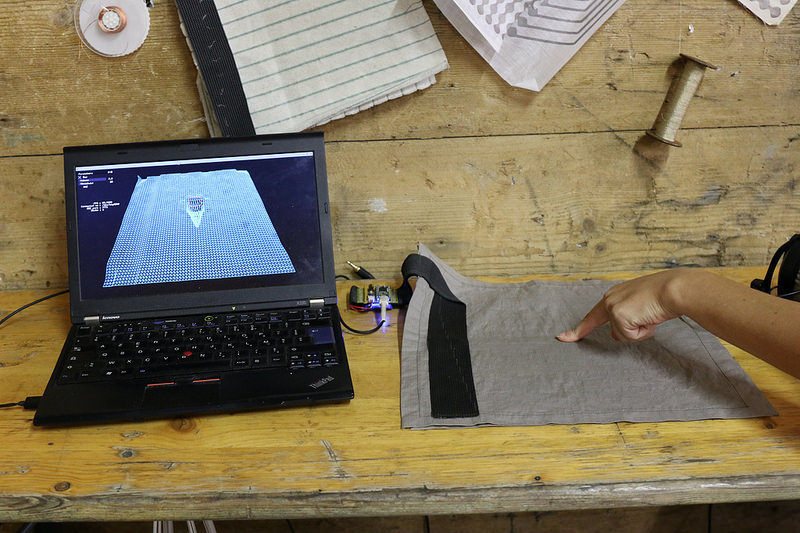
\includegraphics[width=\columnwidth]{figures/touch} }
%   \mbox{ \raisebox{3px}{ Visualization of the Robot Skin being touched.} }
}

% Make sure hyperref comes last of your loaded packages, to give it a
% fighting chance of not being over-written, since its job is to
% redefine many LaTeX commands.
\definecolor{linkColor}{RGB}{6,125,233}
\hypersetup{%
  pdftitle={\plaintitle},
%  pdfauthor={\plainauthor},
  pdfauthor={\emptyauthor},
  pdfkeywords={\plainkeywords},
  bookmarksnumbered,
  pdfstartview={FitH},
  colorlinks,
  citecolor=black,
  filecolor=black,
  linkcolor=black,
  urlcolor=linkColor,
  breaklinks=true,
}

% \reversemarginpar%

\begin{document}

\maketitle

% Uncomment to disable hyphenation (not recommended)
% https://twitter.com/anjirokhan/status/546046683331973120
\RaggedRight{}

% Do not change the page size or page settings.
\begin{abstract}
  UPDATED---\today. This sample paper describes the formatting
  requirements for SIGCHI Extended Abstract Format, and this sample
  file offers recommendations on writing for the worldwide SIGCHI
  readership. Please review this document even if you have submitted
  to SIGCHI conferences before, as some format details have changed
  relative to previous years. Abstracts should be about 150
  words. Required.
\end{abstract}

\keywords{\plainkeywords}

\category{H.5.m}{Information interfaces and presentation (e.g.,
  HCI)}{Miscellaneous}\category{See}{\url{http://acm.org/about/class/1998/}}{for
  full list of ACM classifiers. This section is required.}


\section{Introduction}
We present an art installation consisting of three soft, malleable fabric instruments that users can freely manipulate to play music. Our instruments can be draped over objects, worn, folded, pulled, bent, squished and freely manipulated to produce sound. If worn draped over the body - as a scarf, cape, skirt, bracelet - interesting feedback modalities emerge. The users feel the tactile properties of the fabric in their fingertips, while at the same time feeling the pressure and taps of the fingers through their body. Additionally percussive hits, tones and pads fill the room with sound, leading to a multisensory experience involving the entire body.

We are currently bombarded with advertisement telling us to buy the next wearable gadget to be fitter, happier, more productive. However, these devices are typically rigid both in their form and their expression. Their rigid form does not conform to the bodies soft and dynamic shapes, while their functions are typically constrained by a world view focused on productivity and optimization.

Like the wearable technologies currently pushed by large companies, our fabric can also be worn, but instead of helping us to reach our next goal faster and more efficiently, our fabric invites us to rest and explore our bodies. As it is soft it can conform to the shape of the body in different ways, by manipulating the material draped over our bodies, we explore ourselves, while creating an audible, shared musical experience. We designed our fabric for pleasure and self-expression as a statement opposing a view of ubiquitous computing that turns us into productivity machines.

We present three fabric instruments, with different functions. These mimic the typical composition of a modern pop band. One fabric is an imitation of a drum kit, enabling users to create distinct beats and one-shot sounds by tapping it. Another represents a lead instrument. Touching it creates distinct tones. Depending on the touch, the sound spectrum and pitch of the tone changes allowing users to play haunting melodies on it. A third fabric instrument represents the harmonics section. Throughout the canvas different chords and soundscapes can be explored, creating a backdrop for the other two instruments to explore. These three instruments will be freely accessible to all visitors during the exhibit. As they are very robust, no special training or instruction is required for visitors to explore them.


\section{Related Work}
Electronic textiles have recently received a significant amount of attention with the publication of public Jacquard \cite{jacquard}, however e-textiles and soft circuitry have a much longer history.

Joanna Berzowska published a fabric that could slowly change color in 2004 \cite{berzowska:05} , followed up by investigations into wearable e-textile fashion \cite{berzowska:04}.

Hannah Perner Wilson, published an overview of soft fabric sensors in 2009 \cite{perner-wilson:09} and has since expanded on that work \cite{perner-wilson:10} and has been maintaining an archive of soft textile sensors\footnote{\url{http://www.kobakant.at/DIY}}.

Similar resistive sensing solutions to those in our instrument have been explored by David Holman \cite{holman:14, holman:11}.

There are also several two-dimensional keyboard projects, or "harmonic keyboards" that are similar in layout to our own instruments \cite{lambdoma, seaboard, linnstrument, omnichord}.


\section{History}
The technology used in our textile instruments is based on the work by Maurin Donneaud\footnote{\url{http://Maurin.Donneaud.free.fr}}. Starting in 2005, he was researching the use of textiles as an intuitive way of interact with computers. From the beginning, the aim was to develop technologies with artistic applications: playing music, creating interactive visualizations etc. To achieve this, the tactile properties and affordances of the interface were a primary focus.

Donneaud's sensor is the result of a reflection on the composition and the interpretation of electronic music. A crossover between the world of weaving and electronics. He opted to use textiles, to give a sensual and intuitive dimension to controllers used to play electronic music. Beyond the musical applications, this textile sensor acts as an artificial skin which can provide objects with a sense of touch.

The other inspiration for this installation is TapMe, a wearable percussive kit designed by Cedric Honnet. Designed in Paris in 2011, TapMe supports beat-boxers and rappers in the expansion of their expressivity by amplifying body percussion. A performer wearing TapMe can create different beats and drum hits by hitting thin drum-triggers worn on their body.






\section{Implementation}

This textile sensor was designed with open source collaborative development in mind. The hardware and software are entirely available and documented on \url{eTextile.org}.


\subsection{Textile}

To detect position of touch points, the conductive textile is sliced both in vertical (x) and horizontal (y) strips (see Figure \ref{fig:inside}).
To measure the pressure intensities (z), the sensor uses conductive and piezoresistive textiles (see explanations in next subsection).

\begin{figure}[h!]
    \centering
    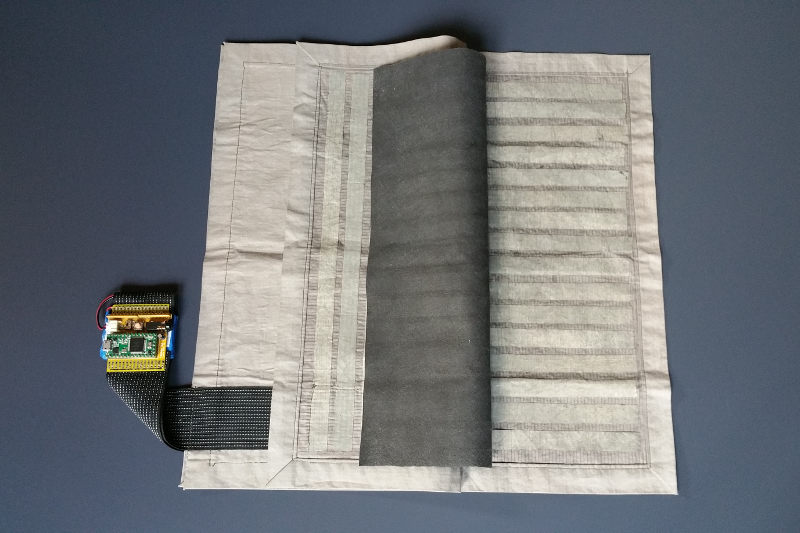
\includegraphics[width=\columnwidth]{figures/inside}
    \caption{The vertical and horizontal stripes of conductive fabric.}\label{fig:inside}
\end{figure}

The piezoresistive textile used for now is made by Eeonyx\footnote{\url{http://eeonyx.com}}, its resistance of 20K ohms per square give a good pressure range and power consumption compare to other possible resistive layers such as velostat\footnote{\url{http://www.lessemf.com/plastic.html}}.


\subsection{Electronics}

Teensy board
piezoresistivity picture
voltage divider


\subsection{Software}

\subsubsection{Microcontroller}

performs measures
send data packets
play music

\subsubsection{Computer}

visualization
blob detection
OSC control






\section{The Installation}
The installation can be adopted to the constraints and opportunities of the space available to us. We envision an enclosed and dimly lit space that contains our instruments. Visitors will enter this space, and see our fabric instruments illuminated. The slight illumination of the fabric is intended to invite people to touch it. Once they do the room will light up softly. Each fabric instrument makes the room light up in different ways, each fabric instrument has its own colors.

Visitors will discover that different instruments have different sound qualities. Some instruments will allow for expressive pressure based interactions triggering ambient pads and soundscapes, others can be played much like a harmonic keyboard. Others again will trigger one-shot sounds, enabling percussive sounds and drumming. The soft malleable nature of the instruments allows for interesting explorations not possible with conventional interfaces. For example, while a single touch typically would trigger a single sound or drum hit, if the instrument is folded, visitors can create custom polyphonic soundscapes. Visitors can explore rubbing, rolling, crumbling to create chaotic or non-deterministic sounds, or lay it out flat on an even surface for high-detail interaction.

Our instruments can be draped over objects to create custom shaped instruments. We will bring a small number of wooden and cardboard shape-primitives that can be used for this purpose. An e-textile might be wrapped around a cylindrical object for providing a better grip, or laid out over a concave bowl to allow faster motion between different areas. Different shapes provide different musical affordances.

Finally our instruments can be draped over bodies. This allows us to use our own bodies as instruments, we can amplify body percussion with additional sounds, or we can hug each other to create soundscapes. The ability to drape these instruments over our body allows us to explore what interactive tattoos might feel like, or what other methods of input in soft fabric devices might feel like on the body. Finally it also allows visitors to explore interacting with interfaces on other peoples bodies. This type of expressive on-body input is something that we have very little experience with and this will allow visitors to improve their intuitive understanding of such potential technologies.


\section{Limitations and Future Work}
While the sensor has a very high resolution along the pressure axis, the spatial resolution is limited by the materials and sensing approach. The minimum spacing between individual sensing strips is constrained by the fabrics we use. We have not established the minimum size yet, but anticipate that there will be a material constrained limiting the resolution. Having said that, we have found that software interpolation works quite well, as usually more than one sensing strip is touched at once. We hope to further improve the software filtering by to using trajectory prediction algorithms such as Kalman filters used in the LumoSpheres project \cite{lumospheres}.

The sensing approach also requires a large number of analog inputs on the micro-controller side. Currently the maximum resolution we can obtain is a matrix of 16 by 16. When we create larger fabric, they do not have a higher resolution, as they still use the 16 by 16 sensing strip design. We are current working on a dedicated micro-controller circuit to improve this.

Finally, we are interested in adding actuation for haptic feedback. We have explored using previous experimentations such as BubbleWrap \cite{bubblewrap} or Shade Pixel \cite{shadepixel} however this added too much bulk to the fabric. While we still wish to add haptic feedback, more experimentation is required to decide on a best approach for this.


\section{Conclusion}
We suggest an installtion consisting of three soft fabric instruments which can be used by visitors to control the environment in the form of adapting sound and lighting. The primary intent of the fabric instruments is for collaboratively making music while exploring shapes, materiality and bodies. This can be done by draping the fabric over objects, folding and deforming the fabric, or wearing it on the body. The e-textile itself is open source and improves over similar sensing applications both in terms of robustness and resolution. We are submitting this installation both because we believe it matches the theme of this years art exhibition, and because we believe it will be an engaging experience for people interested in the topics of TEI.


% \balance{}

\bibliographystyle{SIGCHI-Reference-Format}
\bibliography{tei17}

\end{document}

%%% Local Variables:
%%% mode: latex
%%% TeX-master: t
%%% End:
